\documentclass[a4paper,10pt]{article}

\usepackage{graphicx}
\usepackage[ansinew]{inputenc}
\usepackage[spanish]{babel}
\usepackage{enumerate}
\usepackage{pdfpages}
\usepackage{listings}
\usepackage{color}

\lstset{
  language=C,                	  % choose the language of the code
  numbers=left,                   % where to put the line-numbers
  stepnumber=1,                   % the step between two line-numbers.
  numbersep=5pt,                  % how far the line-numbers are from the code
  backgroundcolor=\color{white},  % choose the background color. You must add \usepackage{color}
  showspaces=false,               % show spaces adding particular underscores
  showstringspaces=false,         % underline spaces within strings
  showtabs=false,                 % show tabs within strings adding particular underscores
  tabsize=2,                      % sets default tabsize to 2 spaces
  captionpos=b,                   % sets the caption-position to bottom
  breaklines=true,                % sets automatic line breaking
  breakatwhitespace=true,         % sets if automatic breaks should only happen at whitespace
  title=\lstname,                 % show the filename of files included with \lstinputlisting;
}

\title{	\textbf{Trabajo Pr\'actico \#0: Infraestructura B\'asica}}
\author{
	Fern\'andez Cynthia, \textit{Padr\'on Nro. 91.487}               \\
	\texttt{ cm.fernandez.28@gmail.com }                             \\[2.5ex]
	Quispe Gaston, \textit{Padr\'on Nro. 86.398}                     \\
	\texttt{ gaston.quispe@gmail.com }                               \\[2.5ex]
	Nombre y Apellido de Autor, \textit{Padr\'on Nro. 90.596}        \\
	\texttt{ valeria.mrb@gmail.com }                                 \\[2.5ex]
	\normalsize{1er. Cuatrimestre de 2017}                           \\
	\normalsize{66.20 Organizaci\'on de Computadoras  $-$ Pr\'actica Mi\'ercoles} \\
	\normalsize{Facultad de Ingenier\'ia, Universidad de Buenos Aires}            \\
       }
\date{}

\makeindex

\begin{document}

\maketitle


\thispagestyle{empty}   % quita el n�mero en la primer p�gina


\begin{abstract}
El objetivo de este trabajo pr\'actico inicial es la adquisici\'on de pr\'actica en la utilizaci\'on de herramientas de software, necesarias para el curso de la materia, a trav\'es de la implementaci\'on de un programa que resuelve el problema propuesto.
\end{abstract}

\tableofcontents

\section{Documentaci\'on relevante}

Se decidi\'o implementar el c\'odigo C dentro de un main(). No implementaremos clases ni librer\'ias propias porque la complejidad l\'ogica del programa no lo amerita.\\
Para el control de la versi\'on utilizamos GitHub. Se trabajo con una rama 'dev' local y se hizo push contra el master.\\
Adjuntamos en esta entrega, los casos de prueba (detalladas en la secci\'on correspondiente).\\


\subsection{Algunos detalles de implementaci\'on}

Con respecto a la implementaci\'on de la l\'ogica de detecci\'on de palabras pal\'indromas, provista por la funci\'on int es\_capicua(char* palabra), se utiliza la funci\'on char tolower(char caracter), provista por la librer\'ia ctype, para cumplir con la condici\'on de ser case insensitive.\\
Las formas posibles de interactuar con el programa son:\\
\begin{itemize}
	\item ./a.output -i <nombreArchivoEntrada> -o <nombreArchivoSalida>: esto lee el contenido de archivo de entrada y lo escribe en el de salida
	\item ./a.output -i <nombreArchivoEntrada> : escribe en salida stdout, es decir en la consola.
	\item ./a.output -o <nombreArchivoSalida>:lee entrada stdin. La finalizaci\'on del ingreso de la palabra se identifica al apretar enter. La finalizaci\'on de la ejecuci\'on de la escritura del archivo se identifica con ctr+d.
	\item ./a.output: lee entrada stdin y stdout.
\end{itemize}


\subsection{Asunciones}

De la interpretaci\'on del enunciado y las dudas resueltas en grupo, cabe destacar lo siguiente:\\
\begin{itemize}
	\item Consideramos pal\'indromos palabras de una sola letra
	\item Dado que los espacios no son caracteres incluidos, entendemos que se s\'olo se evaluar\'an palabras pal\'indromas y no frases. El programa no estar\'a dise\~nado para detectar frases pal\'indromas.
	\item El programa no estar\'a dise\~nado para detectar repeticiones, es decir, si se ingresa dos veces la misma palabra a la entrada y \'esta cumple la condici\'on de ser pal\'indroma, se devolver\'a dos veces esa palabra a la salida.
	\item Utilizamos los caracteres inv\'alidos, es decir, aquellos que no est\'an contemplados en los componentes l\'exicos del stream de entrada, como separadores. De modo que si una palabra incluye un car\'acter inv\'alida quedar\'a separada en dos palabras autom\'aticamente.
	Por ejemplo, si ingresamos AA@BB, el sistema tomar\'a como que se ingresaron las palabras AA y BB.
	\item Cuando existe un error de lectura o escritura, se contin\'ua con la ejecuci\'on y se muestra un mensaje de error. Siendo necesario abortar dicha ejecuci\'on con el comando ctrl + d.
\end{itemize}


\section{Comandos para compilar}

Para compilar el programa utilizamos GCC (GNU Compiler Collection) incluido en NetBSD.\\
\\
\begin{enumerate}[1.]
	\item Movemos los archivos del proyecto a compilar al home en NetBSD\\
	\textbf{scp -P2222 -r /home/tporga root@127.0.0.1:~}

	\item El comando que corremos en la terminal para compilar un archivo con extensi\'on .c es:\\
	\textbf{gcc main.c -Wall}\\
	Si no indicamos par\'ametros de salida, se genera, dentro del directorio donde se encontraba el .c, el archivo  a.out. Para ejecutarlo utilizamos el comando ./a.out.\\

	\item Para obtener el c\'odigo en ensamblador corremos la siguiente linea en el shell.\\
	\textbf{gcc -Wall -O0 -S -mrnames main.c}  (genera el main.s).

	\item Para traer los documentos compilados de nuevo a linux:\\
	\textbf{scp -P2222 -r root@127.0.0.1:/home/tporga ~}
\end{enumerate}

\section{Corridas de pruebas}
Las pruebas leen el ejecutable a.out. Se corre el archivo tests.sh para ejecutar todas las pruebas, con el comando bash test.sh.\\
\\
Las pruebas realizadas son:\\
\begin{enumerate}[1.]
	\item PRUEBA: Entrada vac\'ia.\\
	RESULTADO: Salida vac\'ia.\\

	\item PRUEBA: Entrada de dos frases, con caracteres v\'alidos, dos pal\'indromos.\\
	RESULTADO:\\
	Somos\\
	0\\
	Ojo\\

	\item PRUEBA: Entrada de tres l\'ineas, con caracteres v\'alidos, incluyendo gui\'on medio.\\
	RESULTADO:\\
	Ana\\
	amor-Roma\\
	a\\
	Neuquen\\

	\item PRUEBA: Entrada de mil caracteres con un \'unico pal\'indromo.\\
	RESULTADO:\\
	ojo\\

	\item PRUEBA: Entrada de varios pal\'indromos con caracteres inv\'alidos.\\
	RESULTADO:\\
	11\\
	a--a\\
	ojo\_ojo\\
	-----\\
	somos\\
	ab33ba\\

	\item PRUEBA: Entrada de una palabra pal\'indroma dentro de caracteres inv\'alidos.\\
	RESULTADO:\\
	radar\\

	\item PRUEBA:Entrada de pal\'indromos con guiones y n\'umeros.\\
	RESULTADO:\\
	--\\
	\_\_\\
	99899\\
	99\\
	99\\

	\item PRUEBA: Entrada de varios pal\'indromos entre caracteres inv\'alidos en una sola l\'inea.\\
	RESULTADO:\\
	Neuquen\\
	oro\\
	oso\\
	ojo\\
	radar\\
	reconocer\\
	rotor\\
	salas\\

	\item PRUEBA: Entrada de palabras no palindromas entre caracteres inv\'alidos.\\
	RESULTADO:\\
	Salida vac\'ia.\\

	\item PRUEBA: Entrada de caracteres inv\'alidos.\\
	RESULTADO:\\
	Salida vac\'ia-\\
\end{enumerate}

\section{Problemas e inconvenientes que se presentaron durante el desarrollo del trabajo pr\'actico}
Los principales inconvenientes surgieron de la inexperiencia en la utilizaci\'on de las herramientas propuestas para el desarrollo del trabajo pr\'actico. Las enumeramos a continuaci\'on:

\begin{itemize}
	\item Necesidad de instalar Open SSH para generar el t\'unel.
	\item Necesidad de borrar el archivo know\_host para establecer conexi\'on a la ip.
	\item Decidimos no utilizar un IDE ya que la extensi\'on del c\'odigo no iba a superar las 200 líneas. Simplemente utilizamos un editor de texto. En la experiencia nos hubiese resultado \'util tener un herramienta para debuguear.
	\item Los test observados en la secci\'on 5.1 del enunciado no se adaptan a la definici\'on palíndromo que encontramos y, además, es ambigua. Por lo tanto, y en base a respuestas del grupo yahoo, tomamos como que el ejemplo del test donde el 0 no es palindromo es incorrecto.\\
	Los inconvenientes que surgieron a partir de la interpretaci\'on del enunciado fueron resueltas en la subsecci\'on 'Asunciones'.
\end{itemize}

\newpage
\section{C\'odigo Fuente C}
\lstinputlisting{../main.c}

\newpage
\section{C\'odigo MIPS32}
\lstinputlisting{main.s}

\newpage
\section{C\'odigo de pruebas automatizadas}
\lstinputlisting{../tests.sh}

\newpage
\section{Enunciado}

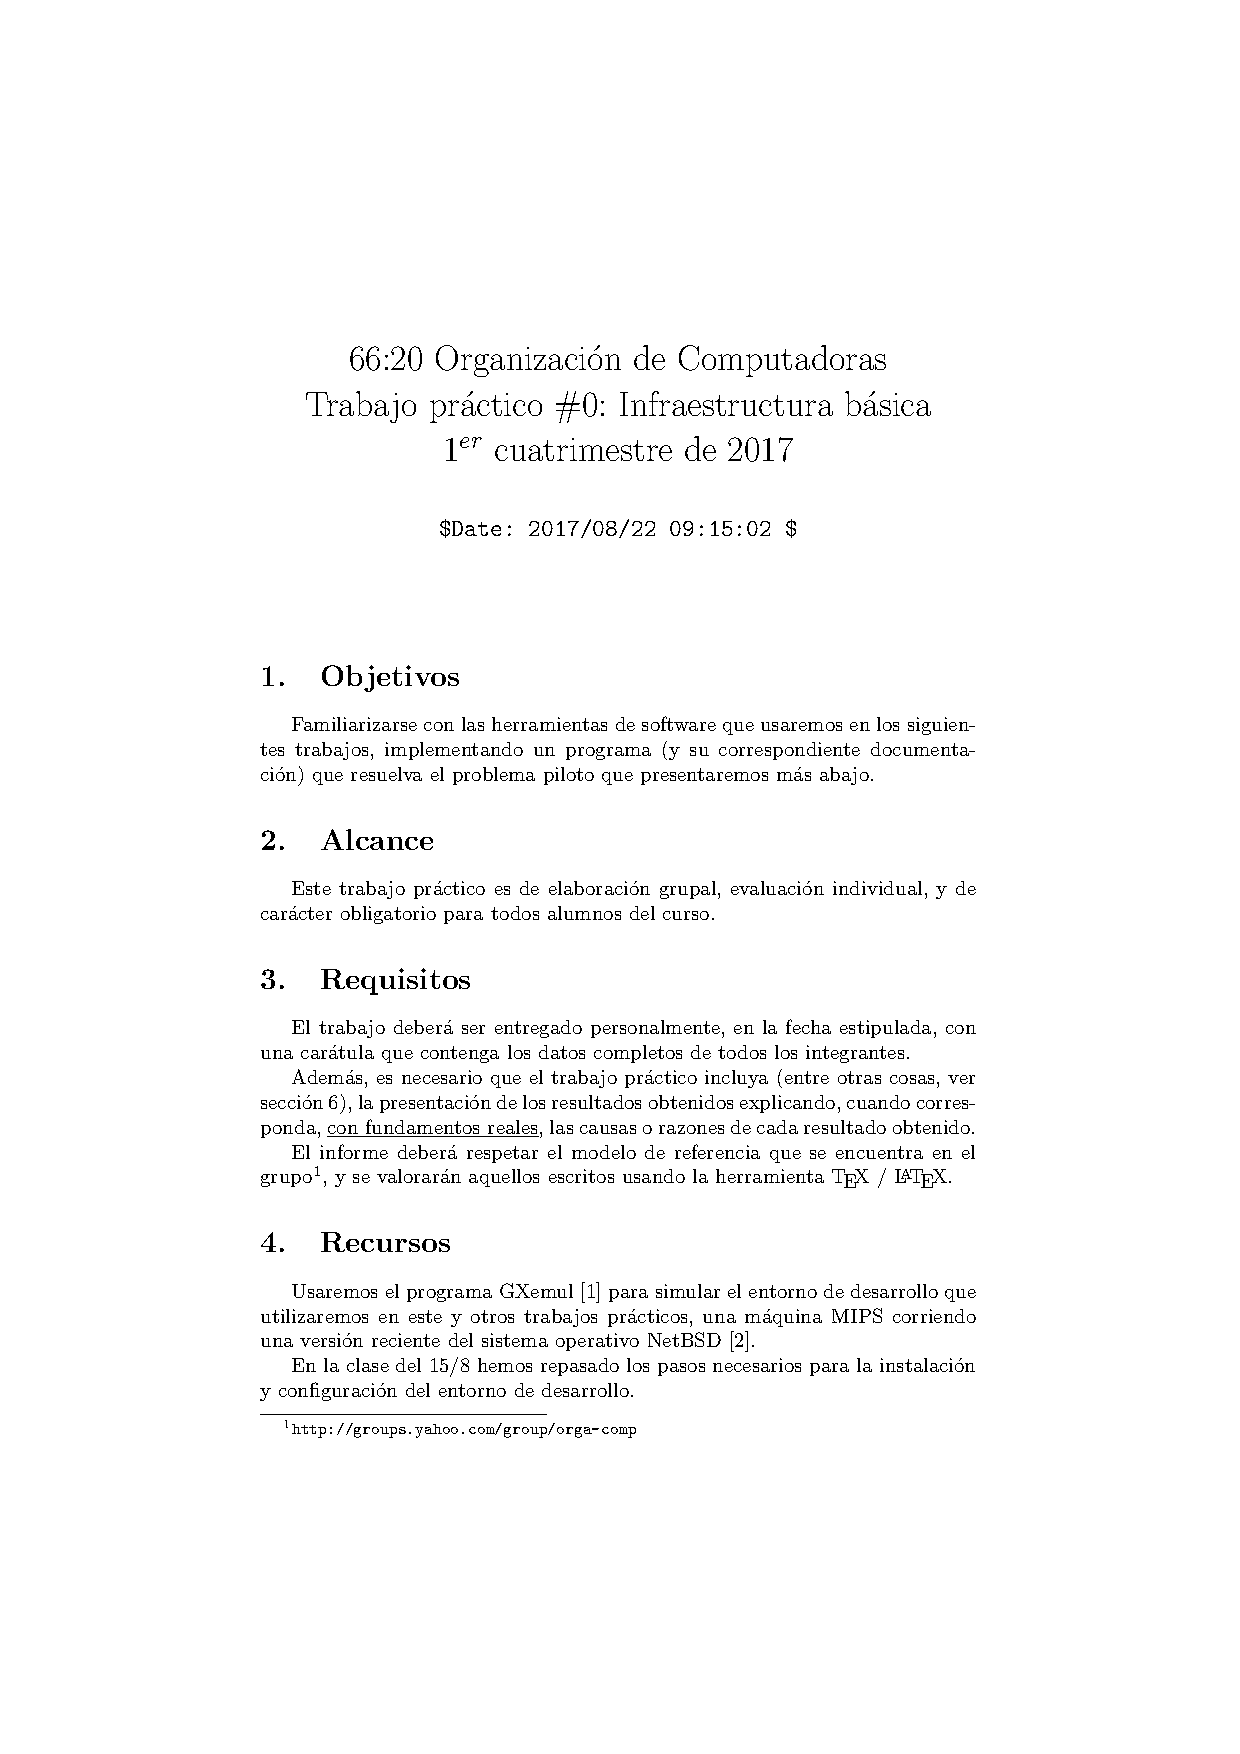
\includepdf[pages=-]{tp0-2017-2q.pdf}

\end{document}
